% !TeX root = ../main.tex

\chapter{相关技术和典型系统}

\section{相关内存数据库索引结构及其并发控制机制}
数据库索引是数据库中最重要的组成部分,而索引的数据结构设计对数据库的性能有重要的影响。
在这里我们介绍几种常见的内存数据库索引结构及其并发控制机制。这里补充一个介绍,因为常用的
数据库描述中都锁都代表逻辑上的锁常用于事务等模块中对记录的互斥访问,是一个逻辑上的概念。
而闩(latch)则表示对数据结构的访问控制,正常情况下只是用来保证数据结构的互斥访问。
但是下面所有的闩和锁都是针对数据结构的锁,保证数据结构的并发访问控制。
因此下面所有的介绍中都对闩和锁不做区分,都代表对索引数据结构的互斥访问。

自20世纪70年代以来,单处理器的性能随着摩尔定律而提高,从而限制了在单台机器上高水平并发执行的需要。但是现在处理器不再提供越来越高的单核性能了。
因此我们需要为多核平台专门设计适应的索引结构。

我们生活在一个高峰值性能的多核世界。单核的速度最多只能适度提高,因此我们需要通过解决至少两个重要方面来更好地利用大量的核心。
1)多核CPU要求高并发性。但是,随着并发水平的提高,悲观锁(latch)更有可能阻塞,限制了可扩展性。
2)良好的多核处理器性能取决于高的CPU缓存命中率。原地更新内存会导致缓存失效,因此如何以及何时进行更新都需要非常小心。

本章内容主要介绍了目前内存数据库中使用的几种索引结构,分别是B+树,跳表,Bw-Tree,Masstree,
同时我们也会简单阐述其常见的并发控制算法。

\section{B+树}
\subsection{B+树简介}
B+树\cite{wu2017empirical}是一个树形结构,是一个n叉排序的树形,每个结点上通常有多个孩子,
一个B+树包含有根结点、内部节点和叶子结点。根结点既可以是一个叶子结点,
也可以是一个同时存在于二个甚至二个以上孩子结点的节点。
而B+树则基本采用了数据库中默认的索引方法,其细节包括:

维基百科在 B+ 树中的节点通常被表示为一组有序的元素和子指针。
如果此B+树的序数(order)是m ,则除了根之外的每个节点都包含最少$ {\displaystyle \lfloor m/2\rfloor } \lfloor m/2\rfloor$ 个元素最多 m-1 个元素,
对于任意的节点有最多 m 个子指针。对于所有内部节点,子指针的数目总是比元素的数目多一个。因为所有叶子都在相同的高度上,
节点通常不包含确定它们是叶子还是内部节点的方式。 每个内部节点的元素充当分开它的子树的分离值。
例如,如果内部节点有三个子节点(或子树)则它必须有两个分离值或元素 a1 和 a2。
在最左子树中所有的值都小于等于 a1,在中间子树中所有的值都在 a1 和 a2 之间,而在最右子树中所有的值都大于 a2。

B+Tree 有如下性质:
\begin{itemize}
\item 查询时间复杂度为 $O(\log _{m}n)$
\item 插入时间复杂度 $O(\log _{m}n)$
\item 删除时间复杂度 $O(\log _{m}n)$
\item 搜索一个范围的键(k 个键)时间复杂度为 ${\displaystyle O(\log _{m}n+k)}$
\end{itemize}

\subsection{B+ 树的多线程同步}

\begin{itemize}

\item 搜索:从根节点开始,获取子节点的读锁,然后释放父节点的读锁;重复这个过程,直到找到目标节点位置。
\item 插入/删除:从根节点开始,获取子节点的写锁;重复这个过程,直到找到目标节点位置;如果子节点是安全的,插入/删除不会引起树结构的变化即父节点不需要调整,可释放所有祖先写锁;乐观的插入/删除是先走搜索获得目标节点的读锁,如果目标节点并不安全,则回归上述从根节点获得写锁的过程。

\end{itemize}

\section{跳表}

\subsection{跳表简介}
Skip List是一种随机化的数据结构,基于并联的链表,其效率可比拟于二叉查找树(对于大多数操作需要O(log n)平均时间)。
基本上,跳跃列表是对有序的链表增加上附加的前进链接,增加是以随机化的方式进行的,所以在列表中的查找可以快速的跳过部分列表(因此得名)。
所有操作都以对数随机化的时间进行。Skip List可以很好解决有序链表查找特定值的困难。

一个跳表,应该具有以下特征:
\begin{itemize}
\item 一个跳表应该有几个层(level)组成;

\item 跳表的第一层包含所有的元素;

\item 每一层都是一个有序的链表;

\item 如果元素x出现在第i层,则所有比i小的层都包含x;

\item 第i层的元素通过一个down指针指向下一层拥有相同值的元素;

\item 在每一层中,-1和1两个元素都出现(分别表示INTMIN和INTMAX);

\item Top指针指向最高层的第一个元素。
\end{itemize}

相对于B+树,跳表有如下优势:

\begin{itemize}
\item  B+ Tree 的插入删除操作有可能会引起树结构的变化,需要从新平衡;与之相对的,跳表插入要简单的多,更加简单高效。
\item B+ Tree 的实现诸如保持树平衡非常复杂;与之相对的,跳表并没有非常复杂的逻辑,实现相对更加简单。
取下一个元素可以再常数时间内,相对于 B+ Tree 的对数时间。
因为链表非常简单,可以很容易的修改跳表结构,以更好地支持诸如范围索引之类的操作。
链表结构使得多线程修改可以仅用 CAS 保证原子性,从而避免重量级的同步机制。
链表的持久化更加简单。
\end{itemize}

\section{Bw-Tree}
\subsection{Bw-Tree 简介}

\begin{figure}[h]
  \centering
  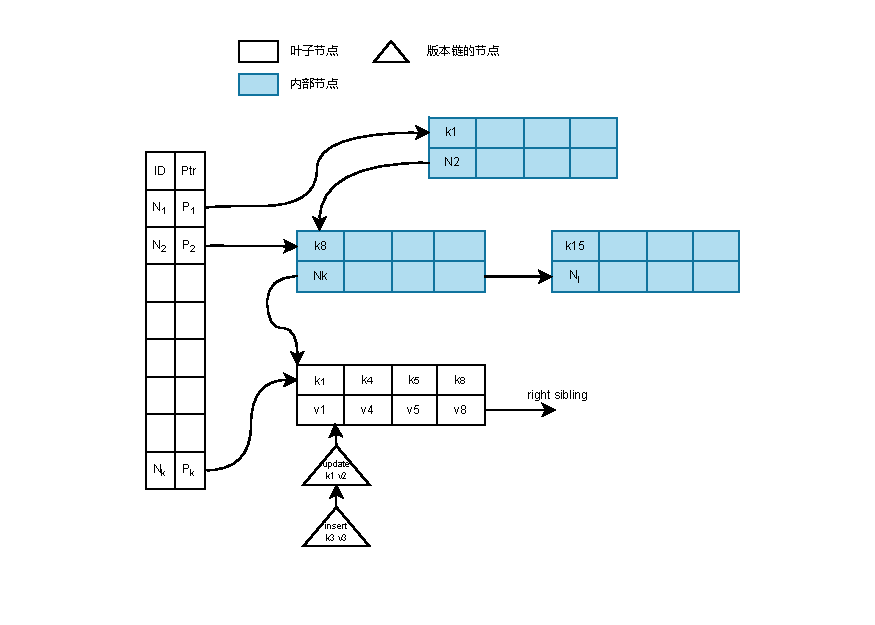
\includegraphics[width=0.9\textwidth]{bwtree.pdf}
  \caption{Bw-Tree的设计概图}
  \label{fig:bwtree}
\end{figure}

Hekaton\cite{larson2011high} 是微软 SQLServer 专门针对 OLTP 应用场景进行优化的数据库引擎,
其索引实现基于 Bw-Tree。Bw-Tree 是一种无需使用任何锁同步的 B+Tree,其主要设计思想如下:

Mapping Table(映射表) 映射表存储内存页的ID与其对应的物理内存地址,
使得线程可以通过访问映射表找到需要方位的内存地址,映射表通过CAS操作来更新。
所有操作不直接修改节点,任何的更新操作都会生成新的数据并且通过指针来指向需要被更新的节点;
新生成的数据所导致的元数据的修改,比如修改映射表都通过 CAS 完成。
垃圾回收机制,Bw-Tree 通过不断新增数据的方式避免直接修改树节点,
在树不断更新的过程中,我们需要对之前旧的数据进行回收,避免版本链的无尽增长降低查询效率。
因此 Bw-Tree 实现了基于 Epoch 的垃圾回收机制:
当一个线程想保护一个它正在使用但是将会被回收的对象,例如检索的时候,
访问了一个内存页,就把当前线程加入 Epoch,当这个线程完成检索页面的操作后,就会退出 Epoch。
通常一个线程在一个epoch的时间间隔内完成一次操作,例如检索。
在线程成功加入 Epoch 的时候,可能会看到将要被释放的老版本的对象,
但不可能看到已经在前一个 Epoch 中释放的对象,因为其在当前 Epoch 中的操作并不依赖上一个 Epoch 中的数据。
因此,一旦所有的线程成功加入Epoch 并完成操作然后退出这个Epoch,回收该 Epoch 中的所有对象是安全的。
由于维护了映射表,和新增数据链,因此树结构调整相对复杂,
不仅仅要调整树,切要保证树结构和映射表之间的关系。

尽管实现非常复杂,Bw-Tree 作为无锁的数据库索引树,有如下优势:
\begin{itemize}
\item No Latch: 实现无锁数据结构十分困难,Bw-Tree 在多线程场景下没有引入任何的latch,
只使用 CAS 指令保证线程同步,因此多核的扩展性优于普通用锁同步的B+Tree。

\item CPU Cache: 由于不直接修改节点而是追加修改补丁,
因此 CPU 缓存不会应为更新数据而失效,因此可以显著提高 CPU 缓存命中率。
微软论文中的数据表明,百分之九十的读操作数据来自 CPU L1/L2 缓存。
\end{itemize}

综上也可以看出Bw-Tree尽可能的不原地修改结构,使用CAS避免悲观锁导致的低扩展性。我们在设计实现乐观级联锁的ART索引时主要参考
Bw-Tree中的去中心化的垃圾回收机制的实现。

\section{Masstree}
\subsection{Masstree 简介}
2012年发表的论文 Cache craftiness for fast multicore key-value storage 提出了 Masstree,其特点如下:

可以理解为B+ Tree 和 Radix Tree 的混合体,即将键切分成多个部分,每个部分为一个节点;
每个节点内部又是一个 B+ Tree,兼顾空间和性能。
Masstree将变长键划分成多个固长部分,每个固长部分可以通过int类型表示,而不是char类型。
由于处理器处理int类型比较操作的速度远远快于char数组的比较,
因此Masstree通过int类型的比较进一步加速了查找过程。固定长度可以设置为 CPU 缓存行长度,以增加 CPU 缓存效率。
每个节点是一个 B+ Tree,因此 CPU 在查询的时候可以将节点所代表的B+ Tree 加载到 CPU 缓存中,
以增加 CPU 缓存命中率\cite{binna2018hot}。

\begin{figure}[h]
  \centering
  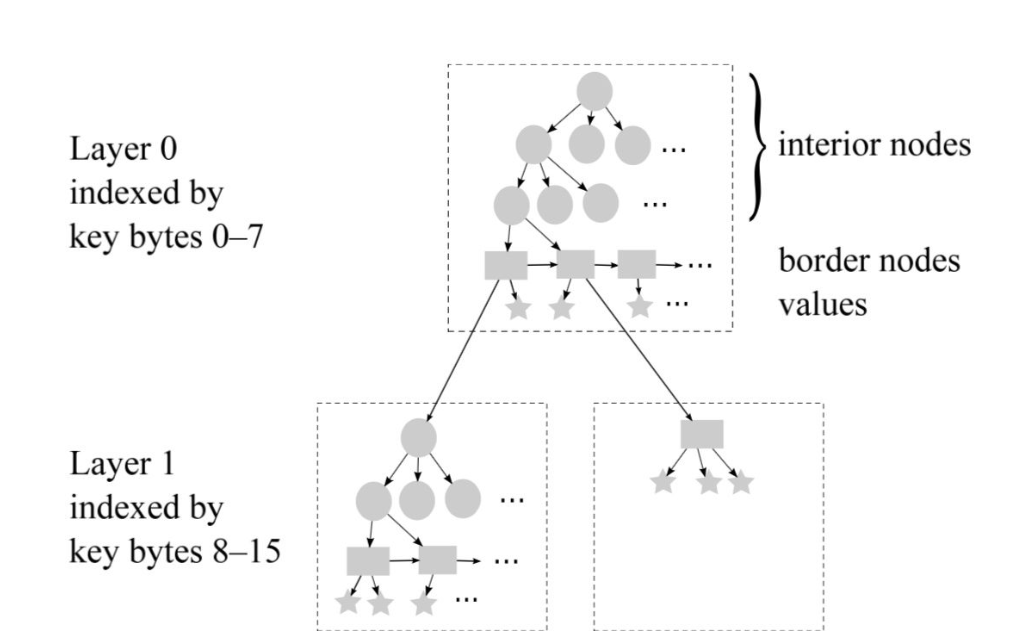
\includegraphics[width=0.9\textwidth]{masstree.png}
  \caption{MassTree的设计概图}
  \label{fig:masstree}
\end{figure}

\subsection{Masstree 并发控制}
MassTree使用细粒度的锁和乐观并发控制来保证高并发。
读并不阻塞写;
写流程要保证并发的读线程不会读到不一致的中间状态;
写写之间用自旋锁互斥。
读操作对比读前和读后记录的"版本号"是否变化或是否被标识为“dirty”或是否被加了写锁,
这些迹象说明有写线程在并发修改记录,读操作重试。

\section{小结}

我们简单介绍了以上几种数据库索引类型以及他们各自的并发控制算法,从上面的索引类型我们可以发现,在内存数据库中
大家普遍采用的是了乐观并发控制,同时这几种数据库都聚焦于提高Cache命中率,避免读操作导致Cache失效,而需要去内存中再读取
数据。同时因为采用乐观并发控制,还需要对于待删除的内存进行管理,不可以立即将内存回收,基本上都是采用的基于Epoch的垃圾回收机制。
这给我们设计和实现基于乐观级联锁的ART索引提供了很大的启发和实现原型。

我们在数据库索引选型时考虑采用ART索引,并使用乐观级联锁处理ART索引的并发控制。我们使用ART索引主要是作为二级索引,主要使用场景是
作为IPTables的索引表。因此我们的ART索引除了提供基本的查询,插入,删除,范围查询接口外,也需要做到对最长前缀匹配的支持。
此外数据库中创建和删除索引等基本的DDL操作也包含在本文的范畴内。

目前商用的DBMS并不是特地为多核CPU而设计,随着核心数的增多,并发控制变得越来越困难,多核并发带来的收益会越来越小,造成实际上的
资源浪费。所以我们主要关注索引结构及其并发算法的可扩展性,这也是为了之后,可以将部分对索引的操作卸载到硬件上所做的必要的预研。

